\wip
\section{Power over Ethernet}
\section{Spannungsregler}
\section{Verstärker}
\subsection{Lautsprecher}
\subsection{Mikrofon}
\section{SMT}
%Entwicklung (zuerst tht, 1960 abgelöst durch smd, erfinder->IBM, Saturn- u. Apollo-Mission)
%Verwendung in Bereich Digitaltechnik, Raumfahrt; Bereiche für tht?
\paragraph{Vorteile:}
\paragraph{Nachteile:}
\subsection{Fehler}
\paragraph{Grabstein-Effekt:} %Bauteil hebt sich beim anlöten von der Platine
\begin{figure}[H]
	\centering
	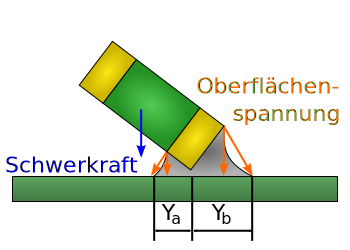
\includegraphics[width=.5\linewidth]{images/technische_grundlagen/grabsteinEffekt.png}%https://upload.wikimedia.org/wikipedia/commons/9/97/Tombstone_Effect_DE.svg
	\caption{Grabstein-Effekt}
\end{figure}

\paragraph{Popcorn-Effekt:} %aufgenommene Luftfeuchtigkeit expandiert beim Heißluftlöten und zerstört das bauteil
\begin{figure}[H]
	\centering
	\includegraphics[width=.5\linewidth]{images/technische_grundlagen/popcornEffekt.jpg}%https://upload.wikimedia.org/wikipedia/commons/9/97/PopcornBGA.jpg
	\caption{Popcorn-Effekt}
\end{figure}
\section{UART}
\section{SPI}